\documentclass[11pt]{scrartcl}
\usepackage{graphicx}
\graphicspath{{./}}
\usepackage[sexy]{evan}
\usepackage[normalem]{ulem}
\usepackage{hyperref}
\usepackage{mathtools}
\hypersetup{
    colorlinks=true,
    linkcolor=blue,
    filecolor=magenta,      
    urlcolor=cyan,
    pdfpagemode=FullScreen,
    }

\renewcommand{\dangle}{\measuredangle}

\renewcommand{\baselinestretch}{1.5}

\addtolength{\oddsidemargin}{-0.4in}
\addtolength{\evensidemargin}{-0.4in}
\addtolength{\textwidth}{0.8in}
% \addtolength{\topmargin}{-0.2in}
% \addtolength{\textheight}{1in} 


\setlength{\parindent}{0pt}

\usepackage{pgfplots}
\pgfplotsset{compat=1.15}
\usepackage{mathrsfs}
\usetikzlibrary{arrows}

\usepackage[most]{tcolorbox}

\begin{document}
		\title{Star Generation WMI Camp - Day 5}
	\author{Orlando Ferrari + Azzam}
	\date{22 March 2024}
	
%	\maketitle
%	\tableofcontents
	
	\section{I Only Update a Bit, Hehe.}
	\begin{enumerate}		
		
		\item A positive number is increased by $60\%$. By what percentage should the result be decreased to return to the original value?
		
		\begin{tabular}{p{2.8cm} p{2.8cm} p{2.8cm} p{2.8cm} p{2.8cm}}
			A. $57.5\%$ & B. $40\%$ & C. $62.5\%$ & D. $50\%$ & E. $37.5\%$
		\end{tabular}
		
		\item If the positive integer $n$ satisfies $5 < \frac{1}{n}+\frac{2}{n}+\frac{3}{n}+\ldots+\frac{15}{n}<8$, how many such $n$'s are there?
		
		\item If $n$ is a whole number, for what values of $n$ is $\frac{80}{n}$ also a whole number?
		
		\item Evaluate $\left(1+\frac{1}{2}\right)\left(1+\frac{1}{3}\right)\left(1+\frac{1}{4}\right)\ldots\left(1+\frac{1}{2023}\right)$.
		
		\item What are the last 3 digits of the sum $1 + 11 + 111 + 1111 + \ldots + \underbrace{111\ldots111}_{70 \text{ digits}}$.
		
		\item The parking lot of a mall has a capacity of $868$ cars. On Thursday, the ratio of the empty parking spots to occupied parking spots is $21 : 41$. How many cars were parked there on that day?
		
		\item The average weight of Alison and Belinda is $26 \ kg$. The average weight of Alison and Carol is $22 \ kg$. The average weight of Belinda and Carol is $24 \ kg$. Find the weight of Carol.
		
		\item In the diagram, $\angle ABC$ and $\angle ADB$ are right angles, $AB = BC$, $BD = 3 \mathrm{cm}$, $AD = 4\mathrm{cm}$. Find the area (in $\mathrm{cm}^2$) of triangle $BDC$.
		\begin{figure*}[h!]
			\centering
			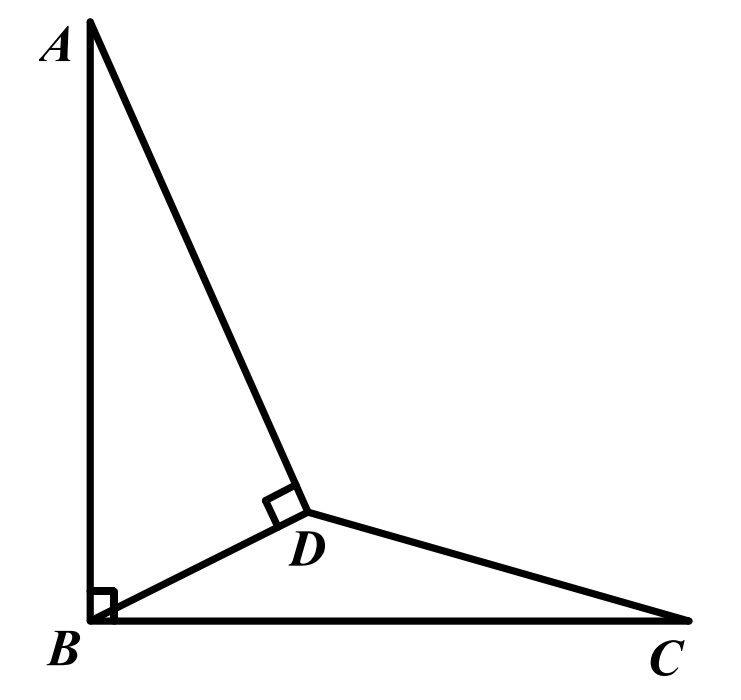
\includegraphics[scale=0.3]{Test For Pelatihan/WMI Camp 2024/Extra Problems V3 Buat Azzam/Images/BDC Area.jpg}
		\end{figure*}
		
		\item In the rectangle $ABCD$, point $E$ is on the side $AB$ while point $F$ is on the side $AD$ such that $BE = \frac{1}{4}AE$ and $DF = \frac{2}{3}AD$. What is the ratio of areas of the rectangle $ABCD$ to triangle $FEC$.
		\begin{figure*}[h!]
			\centering
			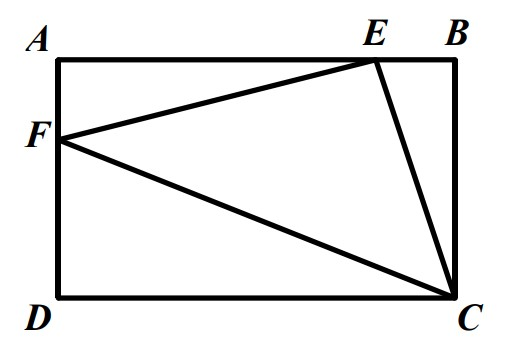
\includegraphics[scale=0.5]{Test For Pelatihan/WMI Camp 2024/Extra Problems V3 Buat Azzam/Images/CEF Area.jpg}
		\end{figure*}
		
		\begin{tabular}{p{2.4cm} p{2.4cm} p{2.4cm} p{2.4cm} p{4cm}}
			A. $30:13$ & B. $40:17$ & C. $48:23$ & D. $24:11$ & E. None of the given
		\end{tabular}
		
		\item How many consecutive digit of 0s are at the end of $8! + 9!$ are there?\\
		\textbf{Note:} $n!$ is defined as $n! = n\times (n-1)\times (n-2)\times \ldots \times 3 \times 2 \times1$, e.g. $5! = 5\times4\times3\times2\times1=120$.
		
		\item (AIMO 2022 Trial) Find $A$ that satisfies the following equation
		\[\scalebox{1.5}{$1+\frac{1}{2+\frac{1}{3+\frac{1}{4+\frac{1}{A}}}} = \frac{139}{97}$}\]
		
		\begin{tabular}{p{2.5cm} p{2.5cm} p{2.5cm} p{2.5cm} p{2.5cm}}
			A. 1 & B. 2 & C. 3 & D. 4 & E. 5
		\end{tabular}
		\item $x$ and $y$ are positive integers, and $\frac{2023+x}{2022+y} = \frac{2023}{2024}$. Find the smallest value of $x+ y$.

		\item (Simulation 1) In the rectangle $ABCD$, point $E$ is on the side $AB$ and point $F$ is on the side $AD$ such that $BE = \frac{1}{5}AB$ and $DF = \frac{1}{9}AF$. What is the ratio of areas of $ABCD$ and $BEFDC$?
				
		\item (Simulation 1) The sum of $7$ positive integers is $63$. Given that $M$ is the largest possible median of these numbers, find the number of posittive factors of $M$.
		\textbf{Note:} The median is the "middle" of the \textbf{sorted} list of numbers.
		
		\item (Simulation 1) Steve is running on a jogging track consisting of 3 circles: X, Y, and Z with a diameter of 36, 18 and 9 meters	respectively. Starting from point P, a “round” of jogging consists of making a full lap around track X, then a full lap around track Y, and finally a full lap around track Z before taking a rest at point P. Steve does several rounds of jogging until he realizes that he has run for $2024\pi$ meter. In which round is Steve now, and at which track?
		\begin{figure*}[h]
			\centering
			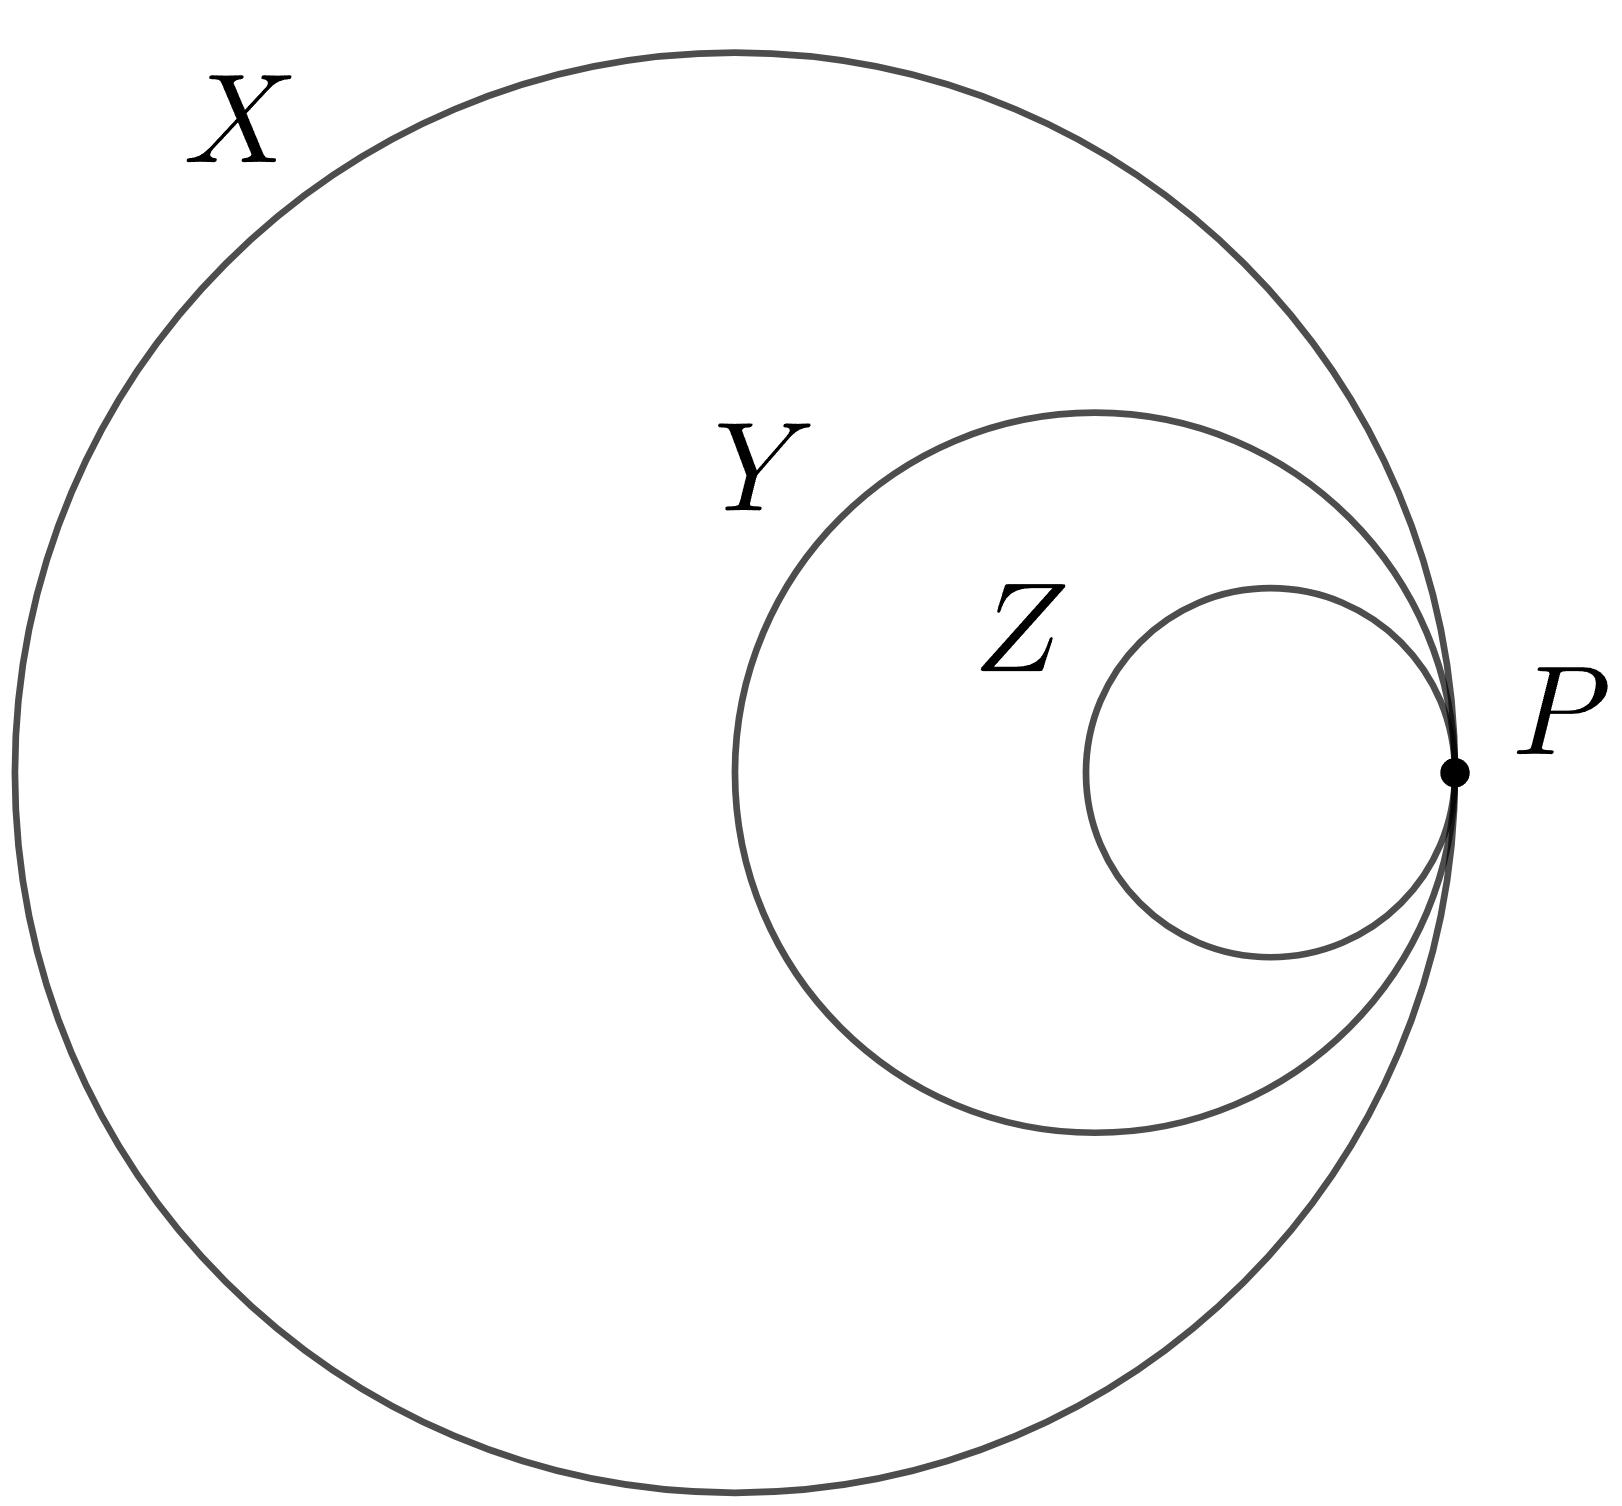
\includegraphics[scale=0.2]{Test For Pelatihan/WMI Camp 2024/Extra Problems V3 Buat Azzam/Images/Ant Goes Crazy-1.png}
		\end{figure*}

\newpage
         \item Given 7 integers. Their mean, median, the only mode, and range are all 7. Among these 7 integers, which option below cannot be the smallest number?
   
   \begin{enumerate}
       \item[(A)] 2
       \item[(B)] 4
       \item[(C)] 5
       \item[(D)] 6
   \end{enumerate}
\vspace{4\baselineskip}

    \item Given 7 integers. Their mean, median, the only mode, and range are all 7. Among these 7 integers, which option below cannot be the smallest number?


    \begin{enumerate}
        \item[(A)] 2
        \item[(B)] 4
        \item[(C)] 5
        \item[(D)] 6
    \end{enumerate}
\vspace{4\baselineskip}

        \item The line graph shows the five baseball teams that the boys and girls in Jeff's class support. Find the team which has the most supporters and the team with the median of the numbers of supporters.

    \begin{center}
        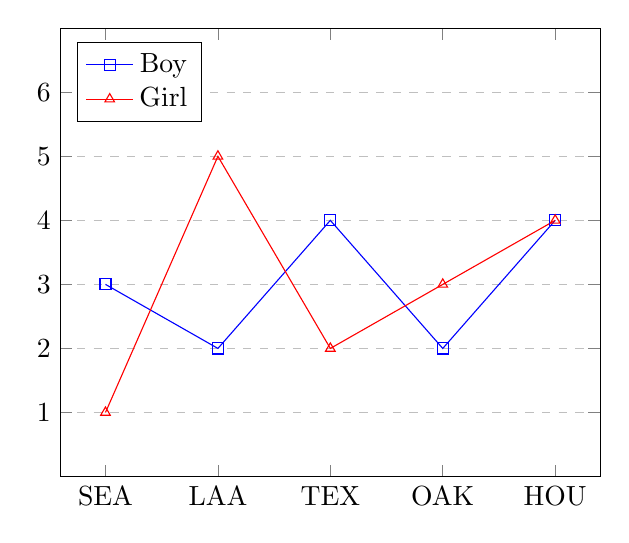
\begin{tikzpicture}
            \begin{axis}[
                xlabel={},
                ylabel={},
                xtick=data,
                xticklabels={SEA,LAA,TEX,OAK,HOU},
                ytick={1,2,3,4,5,6},
                ymin=0,ymax=7,
                legend pos=north west,
                ymajorgrids=true,
                grid style=dashed,
            ]
            \addplot[color=blue,mark=square,]
                coordinates {(0,3)(1,2)(2,4)(3,2)(4,4)};
            \addplot[color=red,mark=triangle,]
                coordinates {(0,1)(1,5)(2,2)(3,3)(4,4)};
            \legend{Boy,Girl}
            \end{axis}
        \end{tikzpicture}
    \end{center}

    \begin{enumerate}
        \item[(A)] LAA, OAK
        \item[(B)] HOU, OAK
        \item[(C)] LAA, TEX
        \item[(D)] HOU, TEX
    \end{enumerate}
    \vspace{4\baselineskip}


    \item Given that 5 workers have to pave a 6km 30m long road in 6 days. How many meters of the road should be done in a day on average?
    \begin{enumerate}
        \item[(A)] 1260
        \item[(B)] 1050
        \item[(C)] 1206
        \item[(D)] 1005
    \end{enumerate}
    \vspace{4\baselineskip}


\item Below is the math test result of a class of 41 students. Find the median and mode of their scores.\\
\begin{tabular}{c|cccccc}
\hline
Score & 50 & 60 & 70 & 80 & 90 & 100\\
\hline
Number of People & 1 & 12 & 8 & 13 & 4 & 3\\
\hline
\end{tabular}
\begin{enumerate}
\item[(A)] Median: 70, Mode: 80
\item[(B)] Median: 80, Mode: 80
\item[(C)] Median: 70, Mode: 70
\item[(D)] Median: 80, Mode: 60
\item[(E)] Median: 80, Mode: 70
\end{enumerate}
\vspace{4\baselineskip}

\item Suppose the 7 numbers given are 3, 2, 5, 5, 6, 2, and 5. If another number 4 is given, which statistic will change?
\begin{enumerate}
\item[(A)] Mean
\item[(B)] Median
\item[(C)] Mode
\item[(D)] Range
\item[(E)] None
\end{enumerate}

	\end{enumerate}
\end{document}










